\subsection{Законы Кеплера}
\paragraph{I-ый закон} \imp{Все планеты движутся по
эллиптическим орбитам, в одном из фокусов которых
находится Солнце.}

Для доказательства первого закона Кеплера введём обозначение: $u \equiv 1/r$, используя его, запишем выражение для модуля момента импульса планеты:
\begin{equation*}
	L = 2 m \sigma = m r^2 \omega = \frac{m \omega}{u^2} = \frac{m}{u^2} \frac{d \theta}{d t},
\end{equation*}
где $\theta$~--- угловая координата в полярной системе координат с центром в центре Солнца.
Выразим $dt$ из полученного выражения.
\begin{equation*}
	dt = \frac{m}{L u^2} \, \d\theta.
\end{equation*}

Найдем теперь первую производную длины радиус-вектора по времени в новых обозначених:
\begin{equation*}
	\frac{d r}{d t} = \frac{d}{d t} \left( \frac{1}{u} \right) = - \frac{1}{u^2} \frac{du}{dt},
\end{equation*}
подставим сюда выражение для $dt$:
\begin{equation*}
	\frac{d r}{d t} = - \frac{1}{u^2} \frac{du \cdot L u^2}{m \d\theta} = - \frac{L}{m} \frac{d u}{d \theta}.
\end{equation*}

Далее получим выражение для второй производной:
\begin{equation*}
	\frac{d^2 r}{dt^2} = \frac{d}{dt} \frac{d r}{d t} = \frac{d}{dt} \left( - \frac{L}{m} \frac{d u}{d \theta} \right) = -\frac{L}{m} \frac{d^2 u}{dt \d \theta},
\end{equation*}
снова воспользуемся выражением для $dt$,
\begin{equation*}
	\frac{d^2 r}{dt^2} = - \frac{L^2	 u^2}{m^2} \frac{d^2 u}{d \theta^2}.
\end{equation*}

Запишем теперь уравнение движения планеты в гравитационном поле Солнца~--- результирующая сила, действующая на планету равна сумме силы гравитационного притяжения и центробежной силы.
\begin{gather}
	m \frac{d^2 r}{d t^2} = - \frac{G M m}{r^2} + m \omega^2 r, \nonumber \\
	- \frac{L^2	 u^2}{m^2} \frac{d^2 u}{d \theta^2} = - GMu^2 + \frac{L^2 u^3}{m^2}, \nonumber\\
	\frac{d^2 u}{d \theta^2} + u = \frac{GM m^2}{L^2}. \label{eq:first-kepler-law-eq}
\end{gather}
Общее решение полученного неоднородного уравнение есть сумма общего решения однородного уравнения 
\begin{equation*}
	\frac{d^2 u}{d \theta^2} + u = 0
\end{equation*}
и частного решения неоднородного уравнения. В качестве частного решения возьмём 
\begin{equation*}
	u(\theta) = \frac{GM m^2}{L^2} = \const.
\end{equation*}
Однородное уравнения является уравнением гармонических колебаний, поэтому его решение можно представить в виде
\begin{equation*}
	u(\theta) = A \cos \theta,	
\end{equation*}
где $A$~--- постоянная интегрирования, определяемая из начальных условий. Общее решение неоднородного уравнения запишется, как
\begin{equation}
	u(\theta) = \frac{GM m^2}{L^2} + A \cos \theta \equiv \frac{1}{r(\theta)}.
	\label{eq:solution-first-kepler-law-eq}
\end{equation}

В качестве начальных условий рассмотрим: $r(0) = s$, $L = m\sqrt{G M h}$, где $s$ и $h$ пока только некоторые расстояния. Подставив выбранные начальные условия в решение~\eqref{eq:solution-first-kepler-law-eq} уравнения~\eqref{eq:first-kepler-law-eq}, получим, что
\begin{gather*}
%	\frac{1}{s} = \frac{GM m^2}{m^2 G M h} + A,\\
	A = \frac{s - h}{sh}.
\end{gather*}
В итоге решение уравнение примет вид
\begin{gather*}
	\frac{1}{r} = \frac{1}{h} + \frac{s - h}{sh} \cos \theta,\\
	r = \frac{sh}{s + (s - h) \cos \theta},\\
	r = \frac{h}{1 + \dfrac{s - h}{s} \cos \theta}.
\end{gather*}
Полученное уравнение является уравнением эллипса в полярных координатах, где $(s - h)/s$~--- эксцентриситет $e$, $h$~--- фокальный параметр $p$, а $\theta$~--- истинная аномалия $\nu$. Это завершает доказательство первого закона Кеплера. Для задачи двух тел доказательство аналогично, достаточно воспользоваться \imp{приведённой массой}.

\paragraph{II-ой закон} \imp{Радиус-вектор планеты за
равные промежутки времени заметает равные площади.}
\begin{equation}
	 \frac{dS}{dt} = \sigma =\frac{L}{2m} = \const = \frac{S_\text{эл}}{T} = \frac{\pi a b }{T}.
\end{equation}
Второй закон Кеплера является прямым следствием \imp{закона сохранения момента импульса}.


\paragraph{III-ий закон} \imp{Квадраты периодов обращения планет
относятся как кубы больших полуосей их орбит.}
\begin{equation}
	\frac{T^2_1}{T^2_2}=\frac{a^3_1}{a^3_2},
\end{equation}
где $a$ --- большая полуось, $T$ --- период обращения.
\begin{figure}[h!]
	\begin{minipage}[b]{0.5\textwidth}
		\centering
		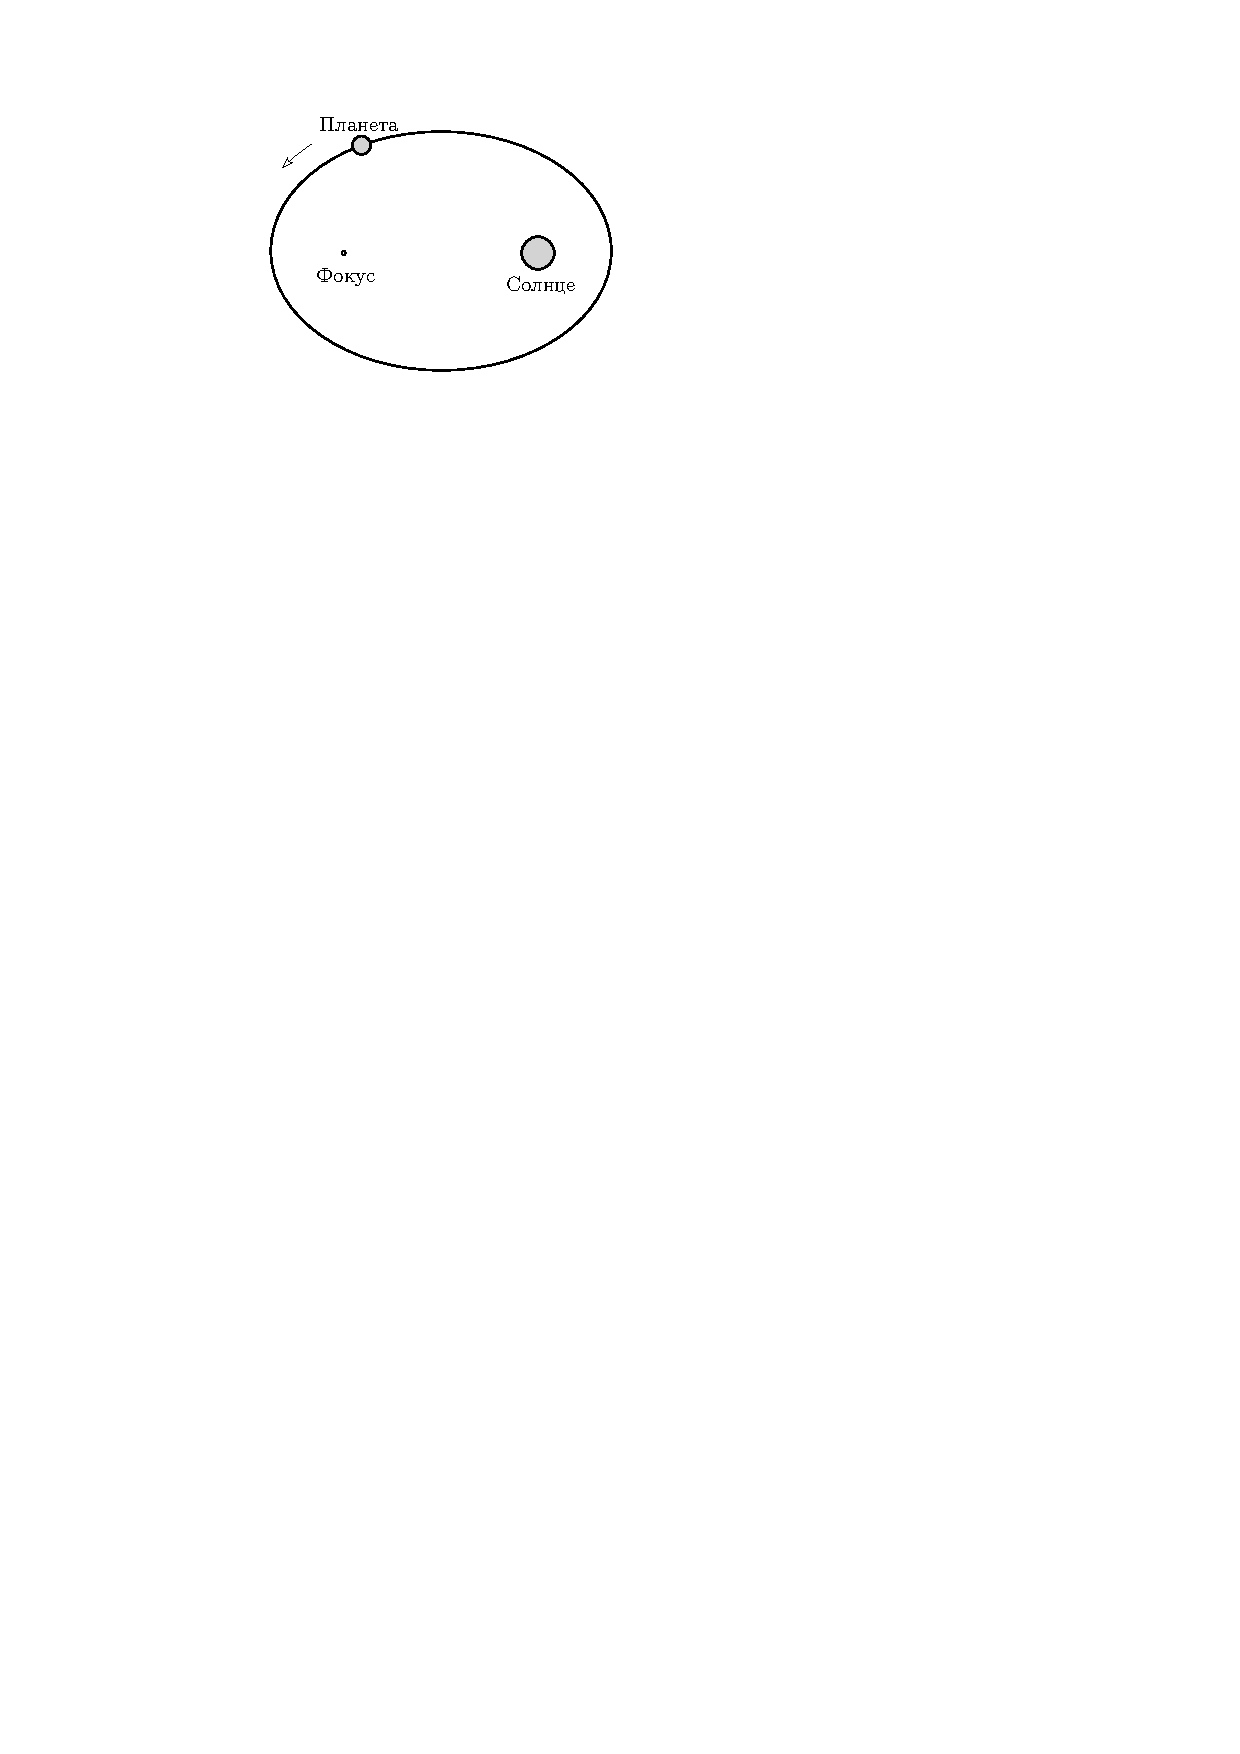
\includegraphics[width = 0.84\textwidth]{first-kepler}
		\caption{Первый закон Кеплера}
	\end{minipage}
	\begin{minipage}[b]{0.5\textwidth}
		\centering
		\begin{tikzpicture}
		\draw (0, 0) -- (1, 1);
%		    \footnotesize
%		    \begin{scope}[yscale=0.6]
%		      \tkzDefPoint(0,0){O};
%		      \tkzDefPoint(2,0){F};
%		      \tkzDefPoint(-20:2.5){A_1};
%		      \tkzDefPoint(40:2.5){B_1};
%		      \tkzDefPoint(120:2.5){A_2};
%		      \tkzDefPoint(140:2.5){B_2};
%		      \tkzDefPoint(-120:2.5){A_3};
%		      \tkzDefPoint(-90:2.5){B_3};
%%		    
%		      \tkzDrawCircle[R](O, 2.5 cm)
%		      \draw [fill=lightgray] (F) -- (A_1) arc(-20:40:2.5) -- cycle;
%		      \draw [fill=lightgray] (F) -- (A_2) arc(120:140:2.5) -- cycle;
%		      \draw [fill=lightgray] (F) -- (A_3) arc(-120:-90:2.5) -- cycle;
%		    
%		      \tkzDefPointBy[homothety=center O ratio 1.04](A_1) \tkzGetPoint{A_1'}
%		      \tkzDefPointBy[homothety=center O ratio 1.05](A_2) \tkzGetPoint{A_2'}
%		      \tkzDefPointBy[homothety=center O ratio 1.05](A_3) \tkzGetPoint{A_3'}
%		     
%		      \tkzDefMidPoint(A_1,B_1) \tkzGetPoint{M_1}
%		      \tkzDefMidPoint(A_2,B_2) \tkzGetPoint{M_2}
%		      \tkzDefMidPoint(A_3,B_3) \tkzGetPoint{M_3}
%		    
%		      \tkzDefPointBy[homothety=center O ratio 1.3](M_1) \tkzGetPoint{M_1'}
%		      \tkzDefPointBy[homothety=center O ratio 1.2](M_2) \tkzGetPoint{M_2'}
%		      \tkzDefPointBy[homothety=center O ratio 1.2](M_3) \tkzGetPoint{M_3'}
%		    
%		      \draw [latex-latex] (A_1') arc(-20:40:2.6);
%		      \draw [latex-latex] (A_2') arc(120:140:2.625);
%		      \draw [latex-latex] (A_3') arc(-120:-90:2.625);
%		    
%		      \draw (M_1') node{$t$};
%		      \draw (M_2') node{$t$};
%		      \draw (M_3') node{$t$};
%
%		      \node at (barycentric cs:F=-0.5,A_1=1,B_1=1) {$S$};
%		      \node at (barycentric cs:F=0.4,A_2=1,B_2=1) {$S$};
%		      \node at (barycentric cs:F=0.4,A_3=1,B_3=1) {$S$};
%		    \end{scope}
		     
%		    \elliparc{0}{0}{3}{1.8}{30}{120}
%
%		    \draw [fill=white] (F) ellipse (0.1);
%		    \filldraw [black] (F) circle (0.01);
%		    \draw [fill=white] ($(O)-(F)$) circle (0.03);
%		    
%		    \node at ($(O) - (F)$)[anchor=north]{$F$};
		\end{tikzpicture}
		\caption {Второй закон Кеплера}
	\end{minipage}
\end{figure}

Получим третий закон Кеплера, из второго. Для этого используем выражения для секториальной скорости через площадь эллипса
\begin{equation*}
    \sigma = \frac{\pi a b}{T} = \frac{\pi a^2 \sqrt{1 - e^2}}{T}
\end{equation*}
 и через момент импульса~--- рассмотрим точку перицентра:
\begin{equation*}
    \sigma = \frac{L}{2m} = \frac{m \sqrt{\dfrac{GM}{a} \cdot \dfrac{1 + e}{1 - e}} \cdot a(1-e)}{2m}.
\end{equation*}
Приравнивая их друг другу имеем:
\begin{gather*}
 \frac{\pi a^2 \sqrt{1 - e^2}}{T}
	= \frac{m \sqrt{\dfrac{GM}{a} \cdot \dfrac{1 + e}{1 - e}} \cdot a(1-e)}{2m},\\
	\frac{4\pi^2 a^4 (1 - e^2)}{T^2}
	= a^2(1-e)^2 \cdot \frac{GM}{a} \cdot \frac{1 + e}{1-e}
\end{gather*}
\begin{equation}
	\frac{T^2}{a^3} = \frac{4\pi^2}{GM}.
\end{equation}

\term{Обобщённый} Ньютоном \term{III-ий закон Кеплера} имеет вид:
\begin{equation}
	\frac{T^2_1( M_1 + m_1)}{T^2_2( M_2 + m_2 )}=\frac{a^3_1}{a^3_2} \quad \Leftrightarrow \quad
	\frac{T^2 ( M + m )}{a^3} = \frac{4 \pi^2}{G},
\end{equation}
где $M_1$ и $M_2$~--- массы центральных тел, $m_1$ и
$m_2$~--- массы обращающихся вокруг них тел. Так как характерная масса планеты
$m$ много меньше массы звезды $M$, полагают $M + m \simeq M$.
